\begin{frame}\frametitle{Quark-Photon Vertex}
\begin{minipage}[r]{0.65\textwidth}
	It is convenient to split the vertex in transverse and longitudinal parts $T_i^{\mu} \; \text{and} \; G_j^{\mu} $ with respect to the incoming photon momentum:
\end{minipage}
\begin{minipage}[r]{0.30\textwidth}
	\hspace{2mm}	
	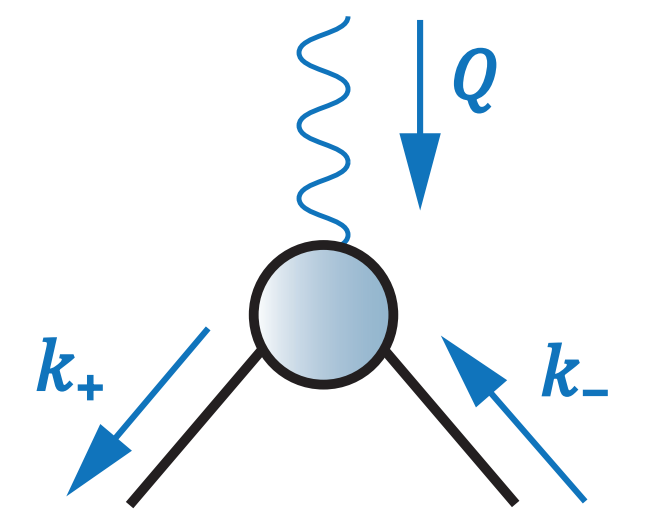
\includegraphics[height=2.2cm, width=3.2cm]{Vertex.png}
\end{minipage}


\begin{equation}
	\Gamma^\mu(k,Q)=\sum_{j=1}^4 g_j(k^2, \omega, Q^2)iG^\mu_j(k, Q)+\sum_{j=1}^8 f_j(k^2, \omega, Q^2)iT^\mu_j(k, Q)
\end{equation}
The quark-photon vertex must satisfy electromagnetic gauge invariance in the form of the
Ward-Takahashi identity (WTI):

\begin{equation}
	Q^\mu\Gamma^\mu(k, Q)=S(k_+)^{-1}-S(k_-)^{-1}
\end{equation}

\end{frame}

\begin{frame}\frametitle{Quark-Photon Vertex}
With this decomposition, the vertex has a charge-conjugation symmetry

\begin{equation}
	\bar{\Gamma}^\mu(k,Q):=-C\Gamma^\mu(-k,Q)^TC^T=\Gamma^\mu(k, -Q) \qquad C=\gamma^4\gamma^2
\end{equation}
\vspace{4mm}
It is easy to show that each $G_j^\mu$, $T_j^\mu$
satisfies the same relation $\Rightarrow$\\ \vspace{3mm} $g_j(k^2, \omega, Q^2)=g_j(k^2, \omega^2, Q^2)$, $\qquad$ $f_j(k^2, \omega, Q^2)=f_j(k^2, \omega^2, Q^2)$\\

\vspace{9mm}

The tensor basis  is free of kinematic constraints $\Rightarrow$ 
\vspace{2mm}
$g_j(k^2, \omega^2,Q^2)$ and $f_j(k^2, \omega^2,Q^2)$ become constant for $Q^\mu\to0$ or $k_\mu\to  0$.

\end{frame}


\endinput
